\newpage
\section{Appendix}
%\thispagestyle{empty}
%\pagenumbering{Roman} 	% R XI and r xi
%\addcontentsline{toc}{section}{Appendix}

%%% table settings
\setcounter{table}{0}
\renewcommand{\thetable}{A\arabic{table}}

\setcounter{figure}{0}
\renewcommand{\thefigure}{A\arabic{figure}}

\begin{ThreePartTable}
\begin{TableNotes}
\footnotesize
\item Anmerkung: Es wurden die Themen vom \textit{Copmarative Agendas Project} übersetzt (Quelle: Comparative Agendas Project 2019).
\end{TableNotes}

\begin{longtable}{p{3cm}p{6,3cm}p{4,5cm}}
 \caption{CAP Topics und verwendete Wörter für die Kategorisierung} \\
 \label{TabCodeBook} \\
 \hline
 Hauptthema & Subthemen & Wörter zwecks Klassifizierung\\
 \hline
Makroökonomie & 
         \textbullet Arbeitslosenquote \newline
         \textbullet allg. Haushaltsprobleme \newline
         \textbullet Inflation \newline
         \textbullet Preise \& Zinsrate \newline
         \textbullet nationales Budget \& Schulden; \newline
         \textbullet Steuerpolitik \newline
         \textbullet Industriepolitik \newline
         \textbullet Preiskontrolle \& Stabilisierung
      & Arbeitslosigkeit, Arbeitslosenquote, Zinsen, Haushaltsschulden, Steuer, Industrie \\ 
\hline
Bürgerrechte & 
         \textbullet Ethnische Minderheiten \newline
         \textbullet Gruppendiskriminierung \newline
         \textbullet Geschlecht \& sex. Diskrimination \newline
         \textbullet Altersdiskriminierung \newline
         \textbullet Diskriminierung von Behinderten \newline
         \textbullet Wahlrechte, Partizipation \& Probleme \newline
         \textbullet Meinungsfreiheit \& Religion \newline
         \textbullet Recht auf Privatsphäre \newline 
         \textbullet Aktivitäten gegen die Regierung 
      & Diskriminierung, Minderheit, Meinungsfreiheit, Religionsfreiheit, Partizipation, Wahlrecht, Gender, Gleichberechtigung, Gleichstellung, Öffentlichkeitsbeteiligung \\
\hline
Gesundheit &
         \textbullet Umfassende Gesundheitsreformen \newline
         \textbullet Versicherungsreform \& Kosten \newline
         \textbullet Regulation der Medikamentenindustrie \newline
         \textbullet Anlagenkonstruktion \& Regulation \newline
         \textbullet Ärztliche Haftung \& Betrug \newline
         \textbullet Gesundheitspersonal \& Ausbildung \newline
         \textbullet Gesundheitsförderung \& Prävention \newline
         \textbullet Kinder und Säuglinge \newline
         \textbullet Geistige Krankheit \& Behinderung \newline
         \textbullet Langzeitpflege \& Sterbenskrankheit
   & Pflege, Pflegeversicherung, Krankenversicherung, Krankenkasse, Arzt, Krankheit, Impfquote, Impfung, Alkoholkonsum, Arzneimittel, Gesundheitsschutz, Medizin, Patienten \\
\hline
Agrarwirtschaft &
         \textbullet Agrarhandel \newline
         \textbullet Subventionen für die Landwirtschaft  \newline
         \textbullet Lebensmittelüberwachung \& Sicherheit \newline
         \textbullet Landwirtschaftliches Marketing \newline
         \textbullet Tier- und Pflanzenkrankheiten \newline 
         \textbullet Schädlingsbekämpfung \& Tierschutz \newline
         \textbullet Fischerei 
   & Agrar, Landwirtschaft, Landwirte, Pflanzenschutzmittel, Glyphosat \\
\hline
Arbeit &
         \textbullet Arbeitssicherheit \& Arbeitsschutz \newline
         \textbullet Personalentwicklung \newline
         \textbullet Angestelltenbonus \newline
         \textbullet Gewerkschaften \newline
         \textbullet Faire Arbeitsnormen \newline
         \textbullet Jugendbeschäftigung \& Kinderarbeit \newline
         \textbullet Elternzeit \& Kinderbetreuung \newline
         \textbullet Wander- und Saisonarbeiter
   & Gewerkschaft, Elternzeit, Kinderbetreuung, Saisonarbeit, Arbeitsschutz, Arbeitssicherheit, Mindestlohn, Mindestlöhne, Streik, Überstunden, Arbeitszeitgesetz, Fachkräftemangel, Arbeitszeit, geringfügige Beschäftigung, befristete beschäftigung, Arbeitsbedingungen, befristeter Beschäftigung, Leiharbeit, Arbeit auf Abruf, Arbeitsunfälle, Stellenabbau, Niedriglöhne \\
\hline
Bildung &
         \textbullet Höhere Bildung \newline
         \textbullet Grund- und weiterführende Bildung \newline
         \textbullet unterprivilegierter Studenten \newline
         \textbullet Berufliche Bildung \newline
         \textbullet Besondere Bildung \newline
         \textbullet Kunst und Geisteswissenschaften
   & Studium, Lehrer, Schule, Universität, Weiterbildung, Geisteswissenschaften, Hochschul \\
\hline
Umwelt &
         \textbullet Trinkwassersicherheit \newline
         \textbullet Müllentsorgung \newline
         \textbullet gefährliche Abfälle \& Chemikalien \newline
         \textbullet Luftverschmutzung \newline
         \textbullet globale Erwärmung \& Lärmbelästigung \newline
         \textbullet Recycling \newline
         \textbullet Umweltgefahren im Innenbereich \newline
         \textbullet Arten- und Waldschutz \newline
         \textbullet Umweltverschmutzung \& Umweltschutz \newline
         \textbullet Land- und Wassereinspeisung
   & Trinkwasser, Recycling, Müll, Luftverschmutzung, Plastik, Klimawandel, Emission, Artenschutz, Stickoxide, Wasserqualität, Umwelt, Klimaschutz, Insekten, Co2-Speicherung, Grundwasser, Tierschutz, Atomtransport, Ökologisch \\
\hline
Energie &
         \textbullet Kernenergie \& Atomkraft \newline
         \textbullet Strom \& Wasserkraft \newline
         \textbullet Natürliche Gase \& Öl \newline
         \textbullet Kohle \newline
         \textbullet Alternativen \& erneuerbare Energien \newline
         \textbullet Energieeinsparung 
  & Kohle, Kohleausstieg, Energie, Atomkraft, Solar, Windenergie, Erneuerbare, Atomstandort \\
\hline
Einwanderung &
         \textbullet Einwanderungsprobleme \newline 
         \textbullet Flüchtlingsprobleme
  & Flüchtlinge, Asyl, Migration, Einwanderer, Einwanderung, Abschiebung, Integration, Familiennachzug, Schutzsuchende, Fluchtursachen, Duldung, Zuwanderung \\
\hline
Transport &
         \textbullet Massentransport \& Sicherheit \newline
         \textbullet Autobahnbau, Wartung \& Sicherheit \newline
         \textbullet Flughäfen, Flugsicherung \& Sicherheit \newline
         \textbullet Eisenbahnverkehr \& Sicherheit \newline
         \textbullet LKW- und Autotransport \& Sicherheit \newline
         \textbullet Maritime Fragen \& Sicherheit \newline
         \textbullet Infrastrukturentwicklung
  & Autobahn, Schienenverkehr, Bahn, Flughafen, LKW, Maut, Mobilität, Schienen, Zugverspätung, Verkehrswende, Verkehrsprojekt, Radverkehr, Verkehrspolitik, Straßenbrücke, Verkehrsminister \\
\hline
Kriminalität &
         \textbullet Wirtschaftskriminalität \newline
         \textbullet organisierte Kriminalität \newline
         \textbullet Illegaler Drogenhandel \& -produktion \newline
         \textbullet Gerichtsverwaltung \newline
         \textbullet Gefängnisse \newline
         \textbullet Jugendkriminalität \& Jugendjustiz \newline
         \textbullet Familienprobleme \newline
         \textbullet Kindesmissbrauch \& Kinderpornografie \newline
         \textbullet Polizei, Feuer \& Waffenkontrolle \newline
         \textbullet Straf- \& Zivilgesetzbuch \newline
         \textbullet Verbrechensverhütung \& -kontrolle 
   & Rauschmittel, Steuerhinterziehung, BND, Bundesnachrichtendienst, Gefängnis, Kindesmissbrauch, Kinderpornografie, Interpol, Kindesentführung, Straftaten, Kriminalität, Sicherungsverwahrung, Tötungsdelikte, Haftbefehl, Bundeskriminalamt, Polizei, Gewalttaten, linksextrem, rechtsextrem, Ermittlungsverfahren, Gefährder \\
\hline
Soziale Wohlfahrt & 
	       \textbullet Nahrungsmittelhilfe \newline
	       \textbullet Armut und Armutshilfe \newline
	       \textbullet Programme für ältere Menschen \newline
	       \textbullet Unterstützung für Behinderte \newline
	       \textbullet Soziale Dienste \newline
	       \textbullet ehrenamtliche Vereinigungen
   & Arbeitslosengeld, Renten, Altersarmut, Pension, Armut, Tafel, Kindergeld, Jobcenter, SGB-II, Vermögensungleichheit, Einkommensungleichheit, Riester-rente, Sozialgesetzbuch, Altersvorsorge \\
\hline
Wohnungsbau &
         \textbullet Wohnungswesen \newline
         \textbullet Stadtwirtschaftliche Entwicklung \newline
         \textbullet Ländliche Wohnungsprogramme \newline
         \textbullet Ländliche wirtschaftliche Entwicklung \newline
         \textbullet Wohnungsbauprogramme \newline
         \textbullet Alten- \& Behindertenwohnungen \newline 
         \textbullet Wohnhilfe für Obdachlose \newline
         \textbullet Sekundäre Hypothekenmarkt
   & Mietpreis, Miete, Wohnung, Obdachlos, Wohnhilfe, Wohnheim, Brachfläche, wohnen \\
\hline
Binnenhandel &
         \textbullet Bankensystem \newline
         \textbullet Finanzinstitutverordnung \newline
         \textbullet Wertpapier- \& Rohstoffverordnung \newline
         \textbullet Verbraucherfinanzierung \newline
         \textbullet Versicherungsverordnung \newline
         \textbullet Konkurs/Insolvenzen \newline
         \textbullet Unternehmenszusammenschlüsse \newline
         \textbullet Probleme kleiner Unternehmen \newline
         \textbullet Urheberrechte \& Patente \newline
         \textbullet Katastrophenhilfe im Inland \newline
         \textbullet Tourismus \newline
         \textbullet Verbraucherschutz \& – betrug \newline
         \textbullet Sport- \& Glücksspielverordnung 
   & Bank, Kartell, Finanzsektor, Verbraucherschutz, Tourismus, Patent, Urheberrecht, Verbraucherschutz, Verbraucherrecht, Fluthilfe, Wettbewerbsbeschränkung, Katastrophenschutz, Finanzmarkt, Kapitalmarkt \\
\hline    
Verteidigung & 
         \textbullet Verteidigungsallianzen \newline
         \textbullet Militärische Intelligenz \newline
         \textbullet Rüstungskontrolle  \newline
         \textbullet Waffenexport \newline
         \textbullet Militär \& Militärgerichte \newline
         \textbullet Zivilschutz \& Heimatschutz \newline
         \textbullet Krieg \& Auslandsoperationen
   & Bundeswehr, Kriegseinsatz, Kriegseinsätze, Nato \\
\hline
Technologie \& \newline Kommunikation &
         \textbullet Satelliten \newline
         \textbullet Telekommunikationsverordnung \newline
         \textbullet Regulationen Rundfunk \newline
         \textbullet Wettervorhersagen  \newline
         \textbullet Computerindustrie \& sicherheit \newline
         \textbullet allgemeine Probleme bzgl. Internet 
   & Internet, Breitband, Telekommunikation, GEZ, Rundfunk, Digitalisierung, Raumfahrt, Cybersicherheit \\
\hline   
Außenhandel &
         \textbullet Streitigkeiten \& Vereinbarungen \newline
         \textbullet Exportförderung \& Regulierung \newline
         \textbullet Int. private Geschäftsinvestitionen \newline
         \textbullet ausländische Investmentgesellschaft \newline
         \textbullet Tarif – \& Einfuhrbeschränkungen  \newline
         \textbullet allg. Einfuhrbestimmungen \newline
         \textbullet Wechselkurs \& verwandte Fragen
   & Handelsabkommen, Export, Import, Zölle, Einfuhrbeschränkung, Einfuhr, Steueroasen, Freihandel, Außenhandel, Export, Waffenexport, CETA, TTIP, transatlantic trade \\
\hline
Internationale \newline Angelegenheiten &
         \textbullet Auslandshilfe \newline
         \textbullet Int. Vereinbarung (über Ressourcen) \newline
         \textbullet Probleme mit Entwicklungsländern \newline
         \textbullet Int. Finanzmärkte \newline
         \textbullet Int. wirtschaftliche Entwicklung \newline
         \textbullet Menschenrechte \newline
         \textbullet Terrorismus \newline
         \textbullet Probleme spezifischer Regionen 
   & Auslandshilfe, Entwicklungsländer, Menschenrecht, humanitäre Hilfe, Brexit, islamischer Staat, Terror, Bürgerkrieg \\
\hline
Regierungs- \newline operationen &
         \textbullet Zwischenstaatliche Beziehungen \newline
         \textbullet Verwaltung staatlicher Immobilien \newline
         \textbullet Regierungseffizienz \& Kontrolle \newline
         \textbullet Skandale der Regierung \newline
         \textbullet Regulierung politischer Kampagnen
   & Sanktionen, Bürokratieentlastung, Bürokratieabbau, bundesanstalt für immobilienaufgaben, Diplomat, Diplomatie \\
\hline
Öffentliche Flächen &
         \textbullet Nationalparks \& Erholung \newline
         \textbullet Denkmäler \& historische Stätten \newline
         \textbullet Waldbewirtschaftung \& öff. Land
   & ausgeschlosen aufgrund \newline extrem weniger Fälle \\
\hline
Kultur & 
         \textbullet allg. kulturelle Probleme
   & ausgeschlosen aufgrund \newline extrem weniger Fälle \\
\hline
\insertTableNotes
\end{longtable}
\end{ThreePartTable}


\begin{figure}[!h]
	\caption{Marginal Effects of Left-Right Scale}
	\label{lrscale_probs}
	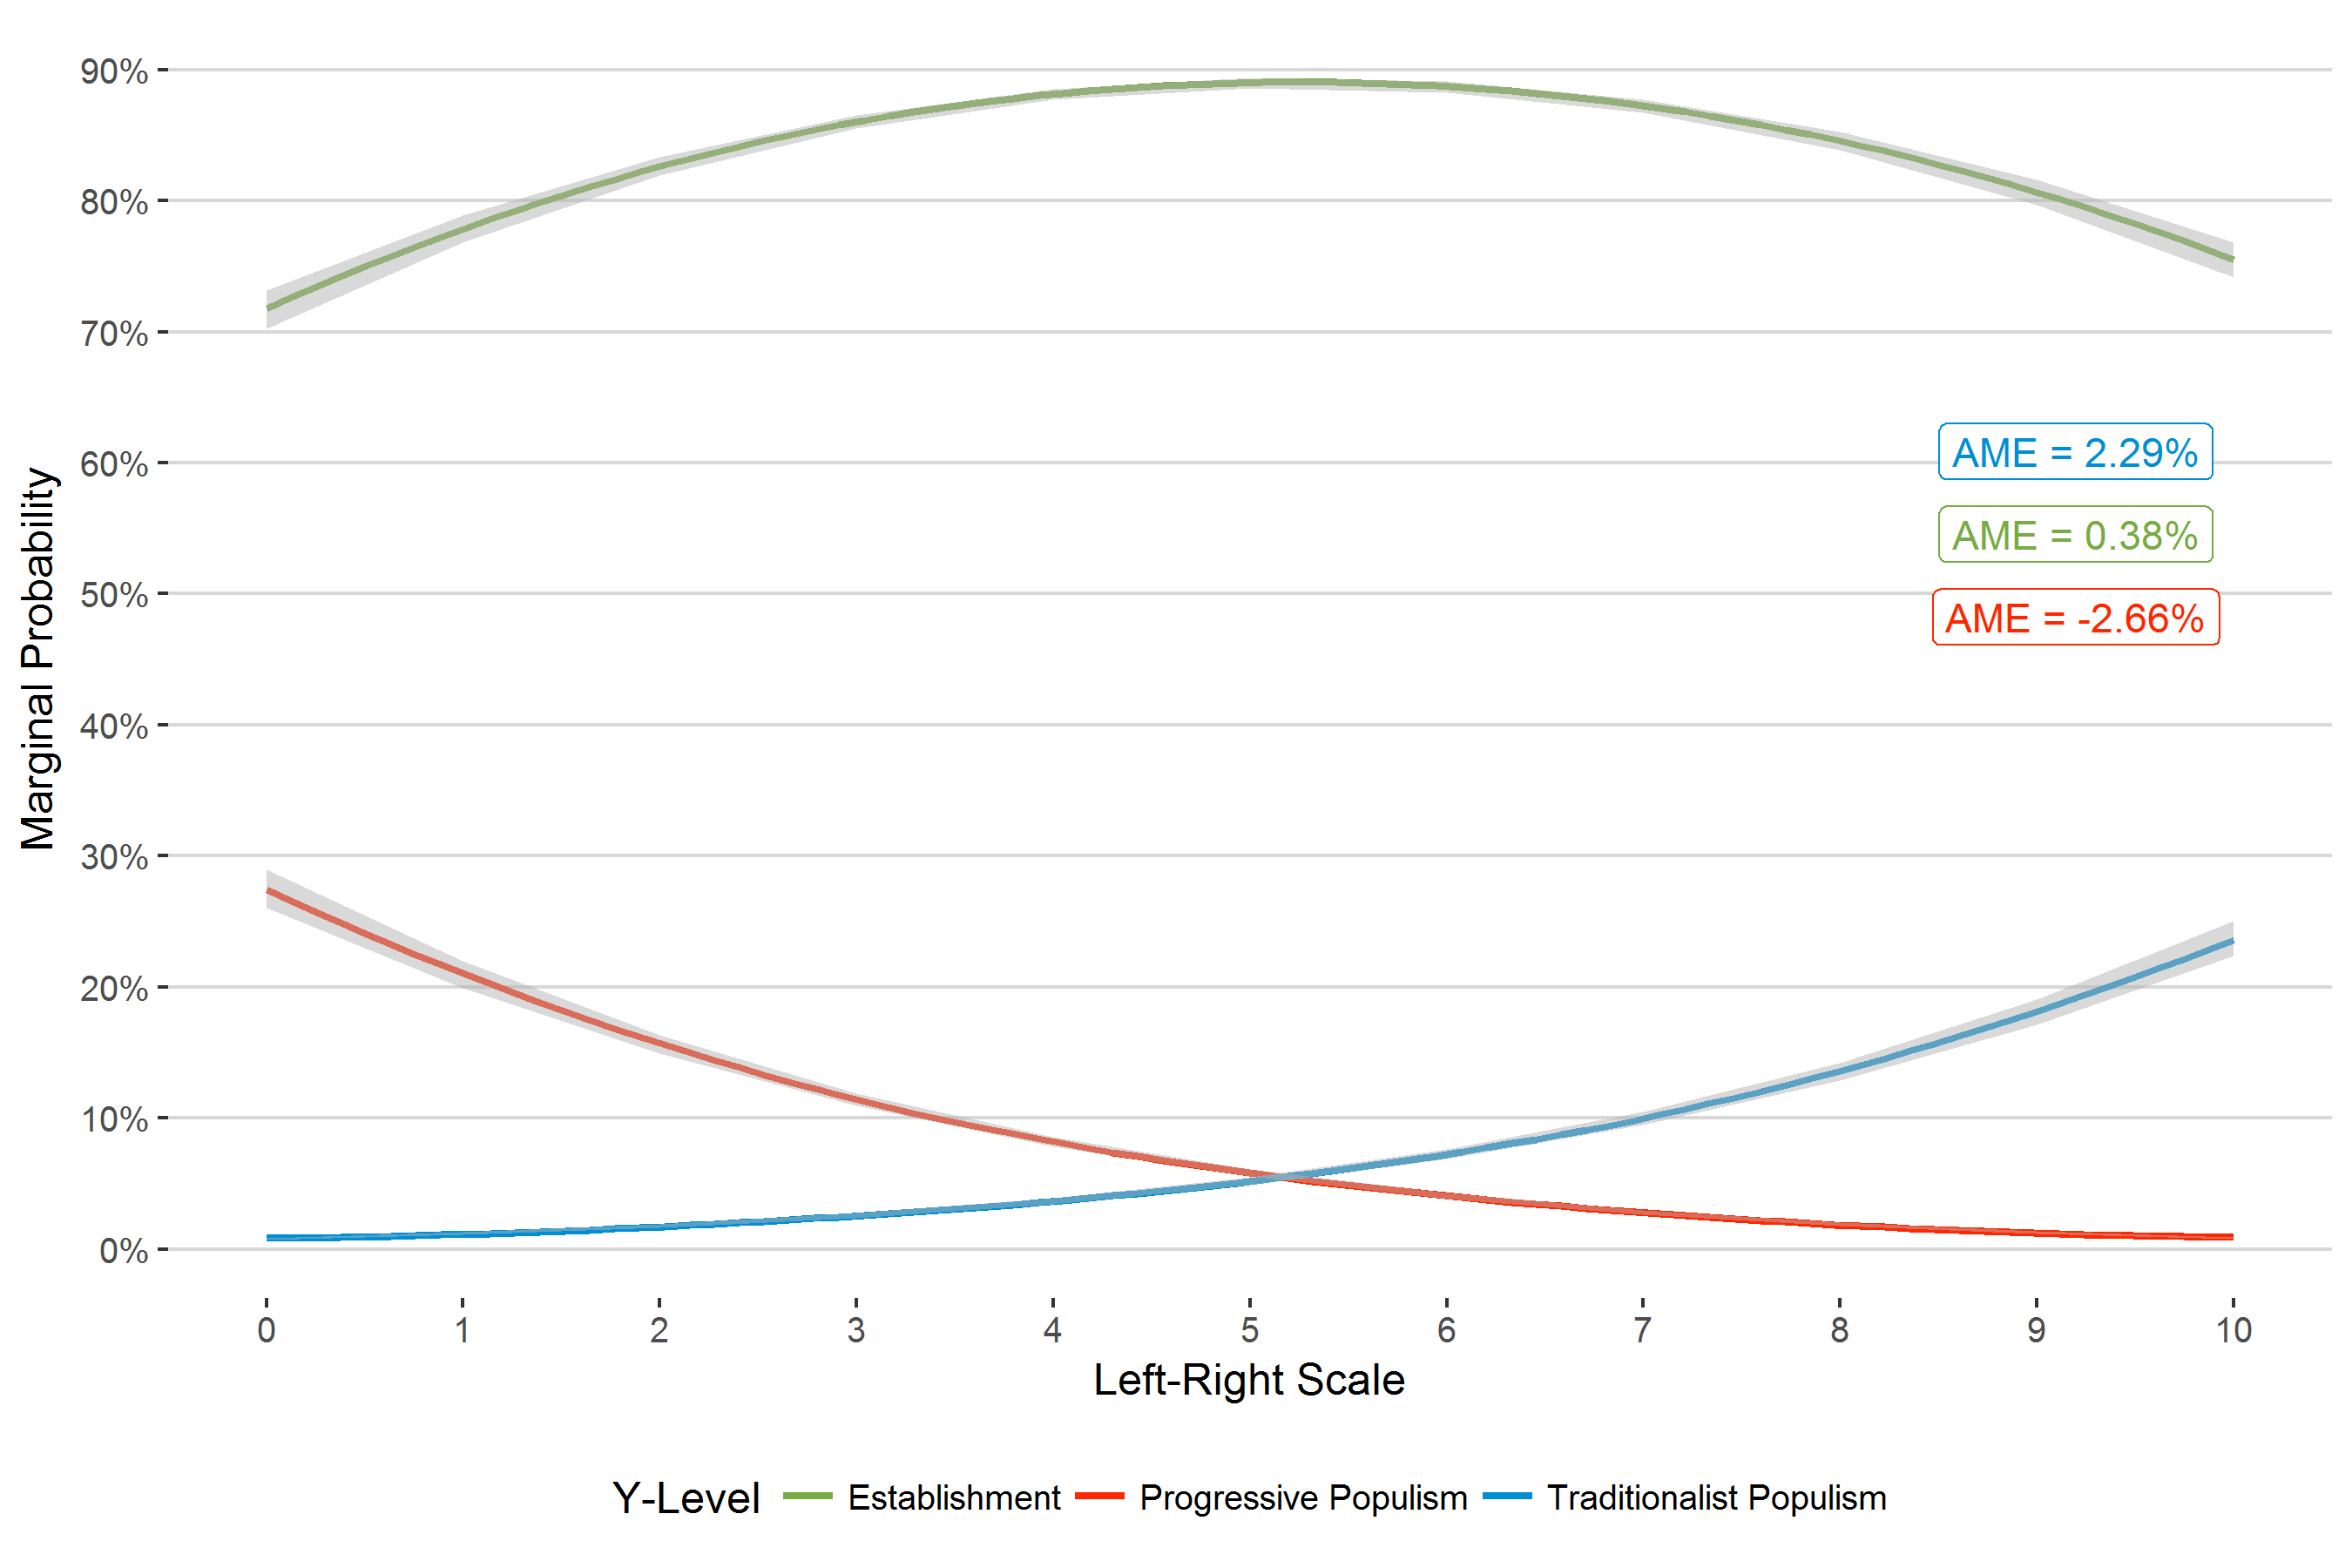
\includegraphics[width=\textwidth]{images/lrscale_probs.png}
	\flushright
	{\scriptsize Based on Model 4. Source: ESS Data Round 5 - 8; N = 68403. \par}
\end{figure}



% \setcounter{table}{1}
% \renewcommand{\thetable}{B\arabic{table}}
% \setcounter{figure}{1}
% \renewcommand{\thefigure}{B\arabic{figure}}


%---------------------------------------------------------------------------%
% Eigenständigkeiterklärung
%---------------------------------------------------------------------------%
\clearpage
\section*{Eigenständigkeitserklärung}
\vspace*{2cm}
\begin{center}
	\begin{minipage}[t]{0.8\textwidth}
		Hiermit versichern wir, dass wir die vorliegende Hausarbeit selbständig und nur mit den angegebenen Hilfsmitteln verfasst haben. Alle Passagen, die wir wörtlich als auch sinngemäß aus der Literatur oder aus anderen Quellen wie z. B. Internetseiten entnommen haben, sind deutlich als Zitat mit Angabe der Quelle kenntlich gemacht.
		
		\vspace*{60mm}
		Stuttgart, 20.03.2019
	\end{minipage}
\end{center}


\end{document}

